\documentclass[border=15pt, multi, tikz]{standalone}
\usepackage{import}
\subimport{../layers/}{init}
\usetikzlibrary{positioning}
\usetikzlibrary{3d} %for including external image 

\def\ConvColor{rgb:yellow,5;red,2.5;white,5}
\def\ConvReluColor{rgb:yellow,5;red,5;white,5}
\def\PoolColor{rgb:red,1;black,0.3}
\def\DcnvColor{rgb:blue,5;green,2.5;white,5}
\def\SoftmaxColor{rgb:magenta,5;black,7}
\def\SumColor{rgb:blue,5;green,15}

\begin{document}
\begin{tikzpicture}
\tikzstyle{connection}=[ultra thick,every node/.style={sloped,allow upside down},draw=\edgecolor,opacity=0.7]
%%%%%%%%%%%%%%%%%%%%%%%%%%%%%%%%%%%%%%%%%%%%%%%%%%%%%%%%%%%%%%%%%%%%%%%%%%%%%%%%%%%%%%%%
%% Draw Layer Blocks
%%%%%%%%%%%%%%%%%%%%%%%%%%%%%%%%%%%%%%%%%%%%%%%%%%%%%%%%%%%%%%%%%%%%%%%%%%%%%%%%%%%%%%%%
% \node[canvas is zy plane at x=0] (temp) at (-3,0,0) {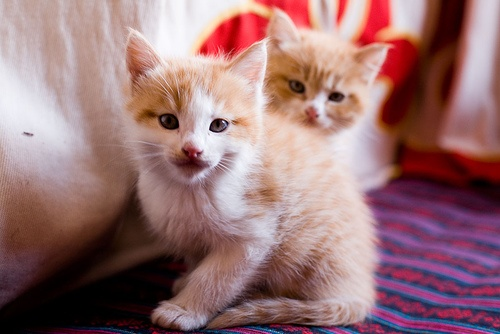
\includegraphics[width=8cm,height=8cm]{cats.jpg}};
% conv1_1,conv1_2,%pool1
\pic[shift={(0,0,0)}] at (0,0,0) {Box={name=cr1,caption=Downsampling,%
        xlabel={{"$n_c$","dummy"}},zlabel=I,fill=\ConvColor,%
        height=40,width=5,depth=40}};
% \pic[shift={(0,0,0)}] at (cr1-east) {Box={name=p1,%
%         fill=\PoolColor,opacity=0.5,height=35,width=1,depth=35}};
% conv2_1,conv2_2,pool2
\pic[shift={(4,0,0)}] at (cr1-east) {Box={name=cr2,caption=First Convolution,%
        xlabel={{"$n_c$","dummy"}},zlabel=I,fill=\ConvColor,%
        height=40,width=5,depth=40}};
% \pic[shift={(0,0,0)}] at (cr2-east) {Box={name=p2,%
%         fill=\PoolColor,opacity=0.5,height=30,width=1,depth=30}};
% conv3_1,conv3_2,pool3
\pic[shift={(2,0,0)}] at (cr2-east) {Box={name=cr3,caption=Second Convolution,%
        xlabel={{"$n_c$","64","64"}},zlabel=I,fill=\ConvColor,%
        height=40,width=5,depth=40}};

\pic[shift={(5,0,0)}] at (cr3-east) {Ball={name=elt0,%
        fill=\SumColor,opacity=0.6,%
        radius=2.5,logo=$+$}};


% %%%%%%%%%%%%%%%%%%%%%%%%%%%%%%%%%%%%%%%%%%%%%%%%%%%%%%%%%%%%%%%%%%%%%%%%%%%%%%%%%%%%%%%%
% %% Draw connections
% %%%%%%%%%%%%%%%%%%%%%%%%%%%%%%%%%%%%%%%%%%%%%%%%%%%%%%%%%%%%%%%%%%%%%%%%%%%%%%%%%%%%%%%%
\draw [connection]  (cr1-east)    -- node {\midarrow} (cr2-west);
\draw [connection]  (cr2-east)    -- node {\midarrow} (cr3-west);
\draw [connection]  (cr3-east)    -- node {\midarrow} (elt0-west);


%%%%%%%%%%%%%%%%%%%%%%%%%%%%%%%%%%%%%%%%%%%%%%%%%%%%%%%%%%%%%%%%%%%%%%%%%%%%%%%%%%%%%%%%
% Residual block

% Vertical line going down
\path (cr1-east) -- (cr2-west) coordinate[pos=0.25] (between1_2) ;
\coordinate (between1_2_down) at ([yshift=-220] between1_2.north west);
\draw [connection]  (between1_2)    -- node {\midarrow} (between1_2_down);

% Horizontal and vertical line going up
\draw [connection]  (between1_2_down) -- node {\midarrow} (elt0-south|-between1_2_down) -- node {\midarrow} (elt0-south);
%%%%%%%%%%%%%%%%%%%%%%%%%%%%%%%%%%%%%%%%%%%%%%%%%%%%%%%%%%%%%%%%%%%%%%%%%%%%%%%%%%%%%%%%


\end{tikzpicture}
\end{document}\grid
